\chapter{Efficient Exact Learning of Loopy CRFs}

\section{Introduction}
As discussed previously, %TODO in the introduction? in pystruct chapter?
 many computer vision algorithms employ conditional random
field models on pixel or superpixel graphs. These graphs, by nature, contain loops,
making exact prediction and loss-augmented prediction in general intractable.
As loss-augmented prediction is a central step in the learning algorithms
discussed in Chapter~\ref{ch:structured_pystruct}, approximate inference leads
to complications in learning.

In this chapter, we investigate the necessity and consequences of these
approximations in the one-slack cutting-plane learning algorithm in the context of semantic
image segmentation. We show that despite inference being deemed intractable in
loopy superpixel models, we are able to learn a pairwise conditional random
field model using a structured support vector machine exactly for this task.
We evaluate our approach on the popular MSRC-21 and Pascal VOC datasets. % and nyu?

The contribution of this chapter is threefold:
\begin{itemize}
    \item We analyze the simultaneous use of multiple approximate inference
        methods for learning SSVMs using the cutting plane method, relating
        approximate learning to the exact optimum. %FIXME really?
    \item We introduce an efficient caching scheme to accelerate cutting plane
        training.
    \item We demonstrate that using a combination of under-generating and exact
        inference methods, we can learn an SSVM exactly in a practical
        application, even in the presence of loopy graphs.
    % also fusion moves is pretty good?
\end{itemize}

While empirically exact learning yields results comparable to those using
approximate inference alone, certification of optimality allows treating
learning as a black-box, enabling the researcher to focus attention on
designing the model for the application at hand.


\section{Related Work}

%Max margin learning for structured prediction was introduced by
%\citet{taskar2003max}, in the form of maximum-margin Markov models. Later, this
%framework was generalized to structural support vector machines by
%\citet{tsochantaridis2006large}. Both works assume tractable loss-augmented
%inference.

%Currently the most widely used method is the one-slack cutting plane formulation
%introduced by \citet{joachims2009cutting}.
%This work also introduced the caching of constraints,
%which serves as a basis for our work. We improve upon their caching scheme, and in
%particular consider how it interacts with approximate inference algorithms.

Recently, there has been an increase in research in learning structured
prediction models where standard exact inference techniques are not applicable,
in particular in the computer vision community.
The influence of approximate inference on structural support vector machine
learning was first analyzed by  \citet{finley2008training}.
\citet{finley2008training} show convergence results for under-generating and
over-generating inference procedures, meaning methods that find suboptimal, but
feasible solutions, and optimal solutions from a larger (unfeasible) set,
respectively.
\citet{finley2008training} demonstrate that over-generating approaches---in
particular linear programming (LP)---perform best on the considered model.
They also show that learning parameters with the LP relaxation minimizes a
bound on the empirical risk when extending the target domain to the relaxed
solutions.
In contrast, we aim at optimizing the non-relaxed objective directly, minimizing
the original empirical risk. This is an important difference, as relaxed solutions
are usually not acceptable in practice.

As using LP relaxations was considered too costly for typical computer vision
approaches, later work employed graph-cuts~\citep{szummer2008learning} or Loopy
Believe Propagation (LBP)~\citep{lucchi2011spatial}. These works use a single
inference algorithm for the whole learning process, and can not provide any
bounds on the true objective or the empirical risk. In contrast, in this chapter
we show how to combine different inference methods that are more appropriate
for different stages of learning.

Recently, \citet{meshi2010learning}, \citet{hazan2010primal} and
\citet{komodakis2011efficient} introduced formulations for joint inference and
learning using duality.
In particular, \citet{hazan2010primal} demonstrate the performance of their
model on an image denoising task, where it is possible to learn a large number
of parameters efficiently.
While these approaches show great promise, in particular for pixel-level or
large-scale problems, they perform approximate inference and learning, and do
not relate their results back to the original SSVM objective they approximate.
It is unclear how they compare to standard structured prediction approaches
on real-world applications.


\section{Learning Structure Support Vector Machines with Approximate Inference}
In this chapter, we will use the 1-slack cutting plane algorithm, as we found this
algorithm to be most suitable for out approach. For reference, the algorithm is outlined
\Secref{one_slac}, Algorithm~\ref{alg_one_slack}. The inference algorithm $I$ is called
in line~\ref{get_cutting_plane}. We investigate algorithms $I$ (often called separation
oracles in the context) that will not yield the exact maximum here.
There are two groups of inference procedures, as identified in
\citet{finley2008training}: under-generating and over-generating approaches.
An under-generating approach satisfies $I(x^i, y^i, \theta) \in
\mathcal{Y}$, but does not guarantee maximality in line~\ref{get_cutting_plane}
of Algorithm~\ref{alg_cutting_plane}. An over-generating approach on the other
hand, will solve the loss-augmented prediction in line~\ref{get_cutting_plane}
exactly, but for a larger set $\hat{\mathcal{Y}} \supset \mathcal{Y}$, meaning
that possibly $I(x^i, y^i, \theta) \notin \mathcal{Y}$.
%We will elaborate on
%the properties of under-generating and over-generating inference procedures in
%Section~\ref{bounds}. %TODO Filler sentence? wat?

\subsection{Bounding the Objective}\label{bounds}
Even using approximate inference procedures, several statements
about the original exact objective (Equation~\eqref{mainequation}) can be
obtained.

Let $o_{\W}(\theta)$ denote objective \eqref{oneslack} with
given parameters $\theta$ restricted to a working set $\W$, as computed in
line~\ref{restricted} of Algorithm~\ref{alg_cutting_plane} and  let
\[
    o^I(\theta) = C\xi' + \frac{||\theta||}{2}^2
\]
when using inference algorithm $I$, that is $o^I(\theta)$ is the approximation of the primal
objective given by $I$. To simplify exposure, we drop the dependency on $\theta$.

Depending on the properties of the inference procedure $I$ used, it is easy to see:
\begin{enumerate}
    \item If all constraints $\hat{y}$ in  $\W$ are feasible, that is generated
        by an under-generating or exact inference mechanism, then $o_{\W}$ is
        an lower bound on the true optimum $o(\theta^*)$.

    \item If $I$ is an over-generating or exact algorithm, $o^I$ is an upper
        bound on $o(\theta^*)$.
\end{enumerate}

We can also use these observations to judge the suboptimality of a given
parameter $\theta$, that is see how far the current objective is from the true
optimum.  Learning with any under-generating approach, we can use 1. to
maintain a lower bound on the objective. At any point during learning, in
particular if no more constraints can be found, we can then use 2., to also
find an upper bound.  This way, we can empirically bound the estimation error,
using only approximate inference.  We now describe how we can further use 1. to
both speed up and improve learning.


\section{Efficient Cutting Plane Training of SSVMs}\label{learning}

\subsection{Combining Inference Procedures}\label{combining}
The cutting plane method described in Section~\ref{cutting_plane} relies only
on some separation oracle $I$ that produces violated constraints when
performing loss-augmented prediction.

Using any under-generating oracle $I$, learning can proceed as long as a
constraint is found that is violated by more than the stopping tolerance
$\epsilon$.  Which constraint is used next has an impact on the speed of
convergence, but not on correctness. Therefore, as long as an under-generating
method does generate constraints, optimization makes progress on the objective.

Instead of choosing a single oracle, we propose to use a succession of
algorithms, moving from fast methods to more exact methods as training
proceeds. This strategy not only accelerates training, it even makes it
possible to train with exact inference methods, which is infeasible otherwise.

In particular, we employ three strategies for producing constraints,
moving from one to the next if no more constraints can be found:
\begin{enumerate*}
    \item Produce a constraint using previous, cached inference results.
    \item Use a fast under-generating algorithm.
    \item Use a strong but slow algorithm that can certify optimality.
\end{enumerate*}

\begin{figure*}
\centering
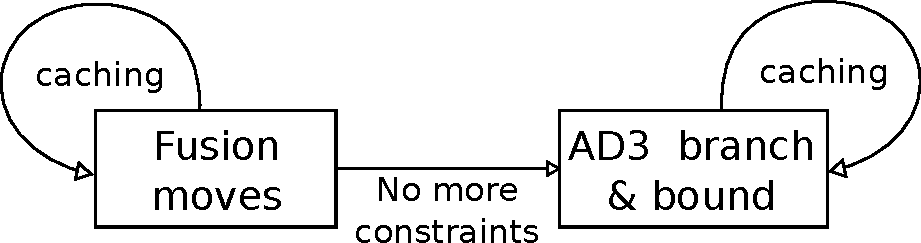
\includegraphics[width=\linewidth]{exact_learning/images/inference_algs}
\caption{%
Illustration of the choice of inference algorithm. During the beginning of learning,
fusion move inference together with caching is used. If no more constraint can be found,
the fusion move algorithm is replaced by AD$^3$ with branch and bound.
\figlabel{scheme_inference_algs}}
\end{figure*}

While using more different oracles is certainly possible, we found
that using just these three methods performed very well in practice.  This
combination allows us to make fast progress initially and guarantee optimality
in the end. Our strategy is visualized in \figref{scheme_inference_algs}
Notably, it is not necessary for an algorithm used as 3) to always produce
exact results. For guaranteeing optimality of the model, it is sufficient that
we obtain a certificate of optimality when learning stops.
% TODO certify optimality != exact...

\subsection{Dynamic Constraint Selection}\label{caching}
Combining inference algorithm as described in Section~\ref{combining}
accelerates calls to the separation oracle by using faster, less accurate
methods. On the down-side, this can lead to the inclusion of many constraints
that make little progress in the overall optimization, resulting in much more
iterations of the cutting plane algorithm. We found this particularly problematic
with constraints produced by the cached oracle.

We can overcome this problem by defining a more elaborate schedule to switch
between oracles, instead of switching only if no violated constraint can be
found any more. Our proposed schedule is based on the intuition that we only
trust a separation oracle as long as the current primal objective did not move
far from the primal objective as computed with the stronger inference
procedure.

%More precisely, let $o_{\W}(\theta)$ denote objective \eqref{oneslack} with
%given parameters $\theta$ restricted to a working set $\W$, as computed in
%line~\ref{restricted} of Algorithm~\ref{alg_cutting_plane} and  let
%\[
    %o^I(\theta) = C\xi' + \frac{||\theta||}{2}^2
    %\]
%when using inference algorithm $I$, that is $o^I(\theta)$ is the approximation of the primal

%objective given by $I$. To simplify exposure, we drop the dependency on $\theta$.
In the following, we use the notation of Section~\ref{bounds} and indicate
the choices of oracle $I$ with $Q$ for a chosen inference algorithm and $C$ for
using cached constraints.

To determine whether to produce inference results from the cache or to run the inference algorithm,
we solve the QP once with a constraint from the cache. If the resulting $o^C$ verifies
\begin{equation}\eqlabel{cache_test}
    o^C - o^Q < \frac{1}{2} (o^Q - o_{\W})
\end{equation}
we continue using the caching oracle. Otherwise we run the inference algorithm again.
For testing \eqref{cache_test}, the last known value of $o^Q$ is used, as recomputing it would defy
the purpose of the cache.

It is easy to see that our heuristic runs inference only $O(\log(o^Q -
o_{\W}))$ times more often than the strategy from \citet{joachims2009cutting} in the
worst case.


\section{Experiments}

\subsection{Inference Algorithms}

As a fast under-generating inference algorithm, we used $\alpha$-expansion
moves based on non-submodular graph-cuts using Quadratid Pseudo-Boolean
Optimization (QPBO)~\citep{rother2007optimizing}.  This move-making strategy
can be seen as a simple instantiation of the more general framework of fusion
moves, as introduced by \citet{lempitsky2010fusion}

For inference with optimality certificate, we use the recently developed
Alternating Direction Dual Decomposition (AD$^3$) method of
\citet{martins2011augmented}. AD$^3$ produces a solution to the linear
programming relaxation, which we use as the basis for branch-and-bound.

\begin{table}
    \begin{center}
    \begin{tabularx}{\linewidth}{@{\extracolsep{\fill}}lcc}
        \toprule
                    & Average & Global \\
        \cmidrule{1-3}
    Unary terms only & 77.7& 83.2 \\
    Pairwise model (move making)& 79.6&84.6\\
    Pairwise model (exact)& 79.0 & 84.3\\
        \cmidrule{1-3}
    \citet{ladicky2009associative} & 75.8& 85.0\\
    \citet{gonfaus2010harmony} & 77&  75\\
    \citet{lucchi2013learning} & 78.9& 83.7\\
    \bottomrule
    \end{tabularx}
    \end{center}
    \caption{Accuracies on the MSRC-21 Dataset.  We compare a baseline model,
    our exact and approximately learned models and state-of-the-art
    approaches.\label{msrcacc}}
    
\end{table}


%\subsection{Multi-Label Classification}
%TODO

%\subsection{Snake}
%TODO

\subsection{Semantic Image Segmentation}
% TODO reference auf davor / intro?
Our main application is of course semantic segmentation and object class
segmentation. We evaluate the proposed learning approach on Pascal VOC 2013 and
MSRC-21

We use the same model and pairwise features for the two datasets.
Each image is represented as a neighborhood graph of superpixels.
For each image, we extract approximately 100 superpixels using 
the SLIC algorithm~\citep{achanta2012slic}.

We introduce pairwise interactions between neighboring superpixels, as is
standard in the literature. Pairwise potentials are founded on two
image-based features: color contrast between superpixels, and relative location
(coded as angle), in addition to a bias term.

We set the stopping criterion $\epsilon=10^{-4}$, though using only
the under-generating method, training always stopped prematurely as no violated
constraints could be found any more.

\subsection{Caching}
First, we compare our caching scheme, as described in Section~\ref{combining}, with the
scheme of \citet{joachims2009cutting}, which produces constrains from the cache
as long as possible, and with not using caching of constraints at all.  For this experiment,
we only use the under-generating move-making inference on the MSRC-21 dataset. Times until convergence
are 397s for our heuristic, 1453s for the heuristic of
\citet{joachims2009cutting}, and 2661s for using no cache, with all strategies
reaching essentially the same objective.

Figure~\ref{caching} shows a visual comparison that highlights the differences
between the methods. Note that neither $o^Q$ nor $o^C$ provide valid upper bounds on the objective,
which is particularly visible for $o^C$ using the method of \cite{joachims2009cutting}.
Using no cache leads to a relatively smooth, but slow convergence, as inference is run often.
Using the method of \citet{joachims2009cutting}, each run of the separation oracle is followed by
quick progress of the dual objective $o_\W$, which flattens out quickly. Much time is then spent adding
constraints that do not improve the dual solution.
Our heuristic instead probes the cache, and only proceeds using cached constraints if the resulting
$o^C$ is not to far from $o^Q$.

\begin{figure*}
\centering
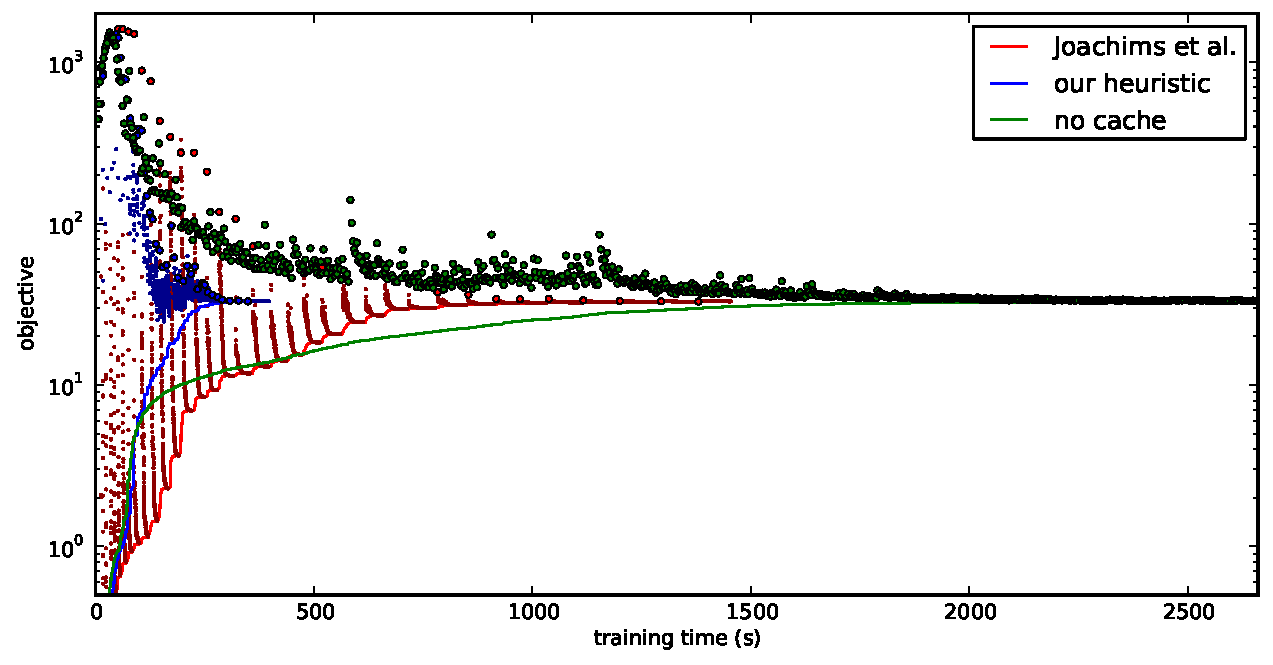
\includegraphics[width=\linewidth]{caching}
\caption{%
Training time comparison using different caching heuristics.
Large dots correspond to $o^Q$, small dots correspond to $o^C$,
and the line shows $o_\W$. See the text for details.\label{caching}}
\end{figure*}
% much simpler model?


\subsubsection{MSRC-21 Dataset}
For the MSRC-21 Dataset, we use unary potentials based on bag-of-words of SIFT
features and color features.  Following \citet{lucchi2011spatial} and
\citet{fulkerson2009class}, we augment the description of each superpixel by a
bag-of-word descriptor of the whole image. To obtain the unary potentials for
our CRF model, we train a linear SVM using the additive $\chi^2$ transform
introduced by \citet{vedaldi2010efficient}. Additionally, we use the unary
potentials provided by \citet{krahenbuhl2012efficient}, which are based on
TextonBoost~\citep{shotton2006textonboost}. This leads to $42 = 2 \cdot 21$
unary features for each node.

The resulting model has around 100 output variables per image, each taking one of 21
labels. The model is trained on 335 images from the standard training and
validation split.

\begin{table}
    \begin{center}
    \begin{tabularx}{\linewidth}{@{\extracolsep{\fill}}lc}
        \toprule
                    & Jaccard \\
        \cmidrule{1-2}
    Unary terms only &  27.5 \\
    Pairwise model (move making)& 30.2\\
    Pairwise model (exact) & 30.4\\
        \cmidrule{1-2}
    \citet{dann2012pottics} & 27.4\\
    \citet{krahenbuhl2012efficient} & 30.2\\
    \citet{krahenbuhlparameter} & 30.8\\
    \bottomrule
    \end{tabularx}
    \end{center}
    \caption{Accuracies on the Pascal VOC Dataset. We compare our approach
    against approaches using the same unary potentials.\label{pascalacc}}
    
\end{table}


\subsubsection{Pascal VOC 2010}
For the Pascal VOC 2010 dataset, we follow the procedure from \citet{krahenbuhl2012efficient}
in using the official ``validation'' set as our evaluation set, and splitting the training set again.
We use the unary potentials provided by the same work, and compare only against methods
using the same setup and potentials, \citet{krahenbuhlparameter} and \citet{dann2012pottics}.
Note that state-of-the-art approaches, some not build on the CRF framework, obtain
around a Jaccard Index (also call VOC score) of 40\% , notably \cite{xia2012segmentation}, who 
evaluate on the Pascal VOC 2010 ``test'' set.


\begin{table}
    \begin{center}
    \begin{tabularx}{\linewidth}{@{\extracolsep{\fill}}lcc}
    \toprule
                    & Move-making & Exact \\
    \cmidrule{1-3}
    Dual Objective $o_\W$ & 65.10 & 67.66  \\
    Estimated Objective $o^I$ &  67.62& 67.66\\
    True Primal Objective $o^E$& 69.92& 67.66\\
    \bottomrule
    \end{tabularx}
    \end{center}
    \caption{Objective function values on the MSRC-21 Dataset}
    \label{msrc_objective}
\end{table}

\subsubsection{Results}
We compare classification results using different inference schemes with
results from the literature. As a sanity check, we also provide results without
pairwise interactions.

Results on the MSRC-21 dataset are shown in Table~\ref{msrcacc}.
We find that our model is on par with state-of-the-art approaches, implying
that our model is realistic for this task. In particular, our results are comparable to those of
\citet{lucchi2013learning}, who use a stochastic subgradient method with working sets.
Their best model takes 583s for training, while training our model exactly takes 1814s.
We find it remarkable that it is possible to guarantee optimality in time of
the same order of magnitude that a stochastic subgradient procedure with
approximate inference takes. Using exact learning and inference does not increase accuracy
on this dataset.
Learning the structured prediction model using move-making inference alone
takes 4 minutes, while guaranteeing optimality up to  $\epsilon=10^{-4}$
takes only 18 minutes.

Results on the Pascal-VOC dataset are shown in Table~\ref{pascalacc}.
We compare against several approaches using the same unary potentials.
For completeness, we also list state-of-the-art approaches not based on CRF models.
Notably, out model matches or exceeds the performance of the much more involved approaches of
\citet{krahenbuhl2012efficient} and \citet{dann2012pottics} which use the same
unary potentials.
Using exact learning and inference slightly increased performance on this dataset.
Learning took 25 minutes using move-making alone and 100 minutes to guarantee optimality
up to $\epsilon=10^{-4}$.
A visual comparison of selected cases is shown in Figure~\ref{visual}.


The objective function values using only the under-generating move-making and
the exact inference are detailed in Table~\ref{msrc_objective} and Table~\ref{pascal_objective}.
We see that a significant gap between the cutting plane objective and the primal objective
remains when using only under-generating inference.
Additionally, the estimated primal objective $o^I$ using under-generating inference is
too optimistic, as can be expected. This underlines the fact that
under-generating approaches can not be used to upper-bound the primal
objective or compute meaningful duality gaps.

\begin{table}
    \begin{center}
    \begin{tabularx}{\linewidth}{@{\extracolsep{\fill}}lcc}
    \toprule
                    & Move-making & Exact \\
    \cmidrule{1-3}
    Dual Objective $o_\W$ &92.06& 92.24\\
    Estimated Objective $o^I$ & 92.07 &92.24\\
    True Primal Objective $o^E$&92.35& 92.24  \\
    \bottomrule
    \end{tabularx}
    \end{center}
    \caption{Objective function values on the Pascal Dataset.}
    \label{pascal_objective}
\end{table}


\subsection{Implementation Details}
We implemented the described procedure in \pystruct.

We used the SLIC implementation provided by \citet{achanta2012slic} to extract superpixels and
the SIFT implementation in the \texttt{vlfeat} package~\citep{vedaldi08vlfeat}.
For clustering visual words, piecewise training of unary potentials and the
approximation to the $\chi^2$-kernel, we made use of the \texttt{scikit-learn}
machine learning package~\citep{pedregosa2011scikit}.
%TODO implementation details here?
The move-making algorithm using QPBO is implemented with the help of the QPBO-I
method provided by \citet{rother2007optimizing}.
We use the excellent implementation of AD$^3$ provided by the authors of
\citet{martins2011augmented}. 

Thanks to using these high-quality implementations, running the whole pipeline
for the pairwise model takes less than an hour on a 12 core CPU\@. Solving the
QP is done in a single thread, while inference is parallelized over all cores.
 
\section{Summary}
In this chapter we demonstrated that it is possible to learn state-of-the-art
conditional random field models exactly using structural support vector
machines, despite the model containing many loops.  The key to efficient
learning is the combination of different inference mechanisms and a novel
caching scheme for the one-slack cutting plane method, in combination with
state-of-the-art inference methods.

We show that guaranteeing exact results is feasible in a practical setting, and
hope that this result provides a new perspective onto learning loopy models for
computer vision applications.
%
Even though exact learning does not necessarily lead to a large improvement in
accuracy, it frees the practitioner from worrying about optimization and
approximation issues, leaving more room for improving the model, instead of the
optimization.

We do not expect learning of pixel-level models, which typically have tens or
hundreds of thousands of variables, to be efficient using exact inference. However we
believe our results will carry over to other super-pixel based approaches.
Using other over-generating techniques, such as duality-based message passing
algorithms, it might be possible to obtain meaningful bounds on the true
objective, even in the pixel-level domain.

\begin{figure*}
\centering
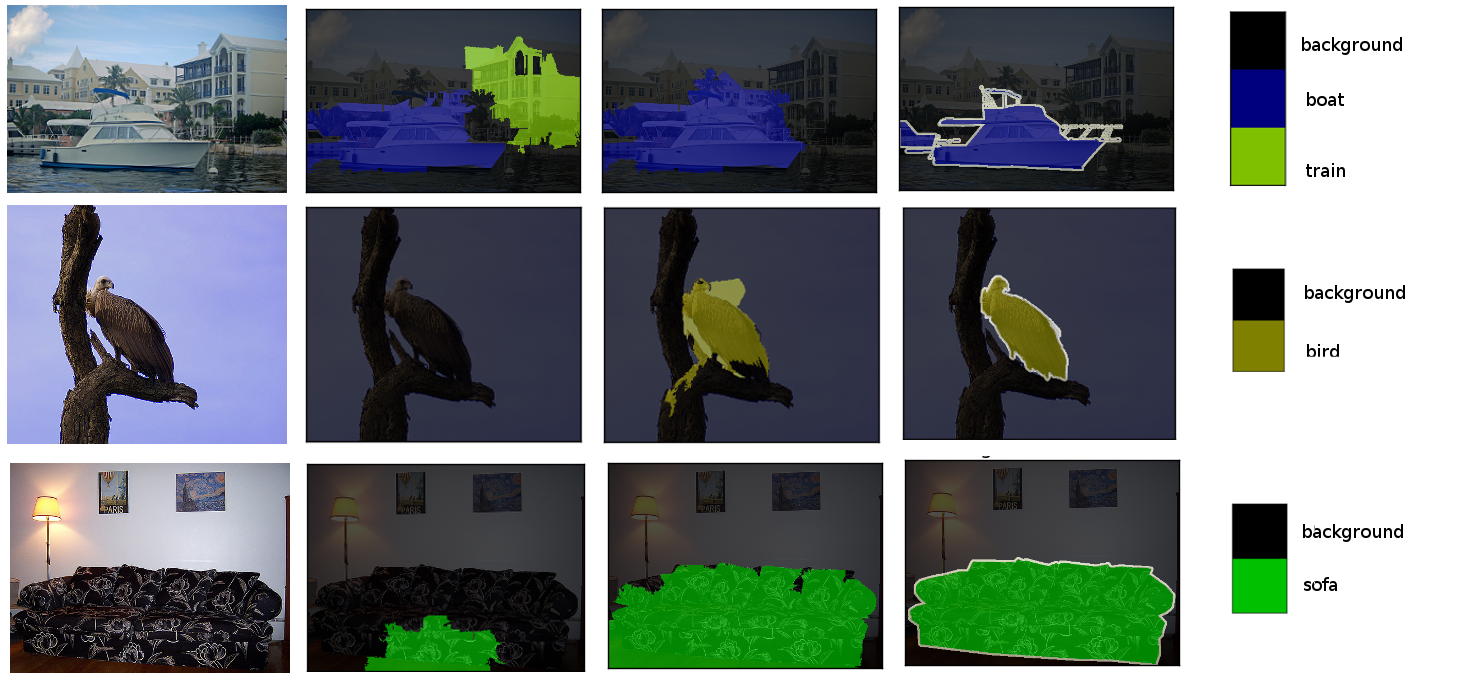
\includegraphics[width=\linewidth]{figure}
\caption{%
    Visual comparison of the result of exact and approximate learning on
    selected images from the test set.  From left to right: the input image,
    prediction using approximate learning, prediction using exact learning, and
    ground truth.
\label{visual}}
\end{figure*}

